\chapter{Languages}

While we may think that computers are just machines, there is an incredible work behind that aims to make some kind of language that computers can understand. It is well renewed that computers act depending on streams of binary code, but that same stream of binary code can be considered as a language, something that the computers "speak" and "think" with. Let's define more in detail this "computers' language".

\begin{definition}{Alphabeth and Strings}
    An \textbf{alphabet} $\Sigma$ is a \textbf{non-empty}, \textbf{finite set}, which contains elements called \textbf{symbols} (or \textbf{characters}). For instance, the following two sets are considered alphabets:
    \begin{itemize}
        \item $\quad \Sigma = \{0, \; 1\}$
        \item $\quad \Sigma = \{a, \; b, \; c, \; \dots, \; x, \; y, \; z \}$
    \end{itemize}
    
    \noindent A \textbf{string} $w$ over an alphabet $\Sigma$ is a \textbf{sequence of symbols}, all belonging to $\Sigma$, which are all written one after the other and aren't separated by other symbols
\end{definition}

\noindent Strings also have different properties, such as a \textbf{length}, a \textbf{reverse} and the possibility to include one or more \textbf{substrings}:
\begin{itemize}
    \item \textbf{Length}: defined as $|w|$, it denotes the \textbf{number of symbols} contained within $w$. If a string has length $0$, then such string is called \textbf{empty string}, and is denoted with $\epsilon$;
    \item \textbf{Reverse}: defined as $w^R$, the reverse is a string which contains all the symbols of $w$ in the reverse order;
    \item \textbf{Substring}: we say that a string $z$ is a substring of $w$ if $z$ appears consecutively within $w$.
\end{itemize}

\begin{example}
    For instance, the string $w = 00101$ has a length of $5$, its reverse is $w^R = 10100$, and has, as possible substrings the following: $001, 10, \epsilon$. Its alphabet is $\Sigma = \{0, \; 1\}$
\end{example}

\noindent When we have two strings $x$ and $y$, we can \textbf{concatenate} them by appending $y$ at the end of $x$. The result is denoted as $xy$. Clearly, the length of the concatenated string is equal to the sum of the length of the two strings ($|xy| = |x| + |y|$). A specific notation $x^k$ denotes the concatenation of string $x$ with itself for $k$ times. So, if $x$ was for instance "$01$", then we would have that
\[ x^0 = \epsilon \quad \quad x^1 = 01 \quad \quad x^2 = 0101 \quad \quad x^3 = 010101 \quad \text{and so on...} \]

\noindent By combining the definitions of concatenation and substring, we can define properly what a \textbf{prefix} and \textbf{suffix} is:
\begin{itemize}
    \item \textbf{Prefix}: we say that a string $x$ is a prefix of a string $z$ if there exists a string $y$ such that $z = xy$. Moreover, we say that $x$ is a \textbf{proper prefix} of $z$ if, additionally, $x \neq z$, so if $y \neq \epsilon$;
    \item \textbf{Suffix}: we say that a string $x$ is a suffix of a string $z$ if there exists a string $y$ such that $z = yx$. Moreover, we say that $x$ is a \textbf{proper suffix} of $z$ if, additionally, $x \neq z$, so if $y \neq \epsilon$.
\end{itemize}

\noindent Given these tools, we can now define what a language is:

\begin{definition}{Language}
    A \textbf{language} is a \textbf{set of strings}. It is also defined as \textbf{prefix-free} if no member is a proper prefix of any other member
\end{definition}

\noindent Languages can follow an order. There are different types of orders, one of which is the \textbf{lexicographic order}, which is defined by the order of the alphabet; we can think of it as the familiar dictionary order. Another order is the \textbf{shortlex order} (or \textbf{string order}), which is the same of the lexicographic order with the exception that shorter strings precede longer strings.

\section{Deterministic Finite Automata (DFA)}

We know that sometimes circuits can use the output from a given combination of inputs as input for the next output. In that case, we talk about circuits with states, or more specifically, we talk about \textbf{automata}.

\begin{definition}{Deterministic Finite Automaton (DFA)}
    We define a \textbf{finite automaton} as a tuple of 5 elements $(Q, \; \Sigma, \; \delta, \; q_{0}, \; F)$, where:
    \begin{itemize}
        \item $Q$ is a finite set, denoting the \textbf{states} that the automaton can reach;
        \item $\Sigma$ is a finite set, denoting the \textbf{alphabet} of the automaton;
        \item $\delta$ is a function, called \textbf{transition function}, which given $Q$ and $\Sigma$ returns the set of next states $Q'$;
        \[ \delta \; : \; Q \times \Sigma \longmapsto Q'  \]
        \item $q_{0} \in Q$ is a state, and denotes the \textbf{starting state} of the automaton;
        \item $F \subseteq Q$ is a finite set, denoting the set of \textbf{accepted states} (or \textbf{final states}). An accepted state tells the automata if a string can be accepted or not.
    \end{itemize}
\end{definition}

\noindent Let's make an example:

\begin{example}
    Consider the following tuple: 
    \[ (\{ q_{1}, \; q_{2}, \; q_{3} \}, \{ 0, \; 1 \}, \delta, \; q_{1}, \; q_{2}) \]
    
    \noindent It denotes that we have 3 possible states $\{ q_{1}, \; q_{2}, \; q_{3} \}$, the alphabet is made of 2 symbols, $\{ 0, \; 1 \}$, the starting state is $q_{1}$, the final state is $q_{2}$ and the transition function is $\delta$. Such transition function could be the following: 
    \begin{center}
        \begin{tabular}{c|c c}
            & 0 & 1 \\
            \hline
            $q_{1}$ & $q_{1}$ & $q_{2}$ \\
            $q_{2}$ & $q_{3}$ & $q_{2}$ \\
            $q_{3}$ & $q_{2}$ & $q_{2}$
        \end{tabular}
    \end{center}
    
    \noindent We can represent it visually as follows:
    \begin{center}
        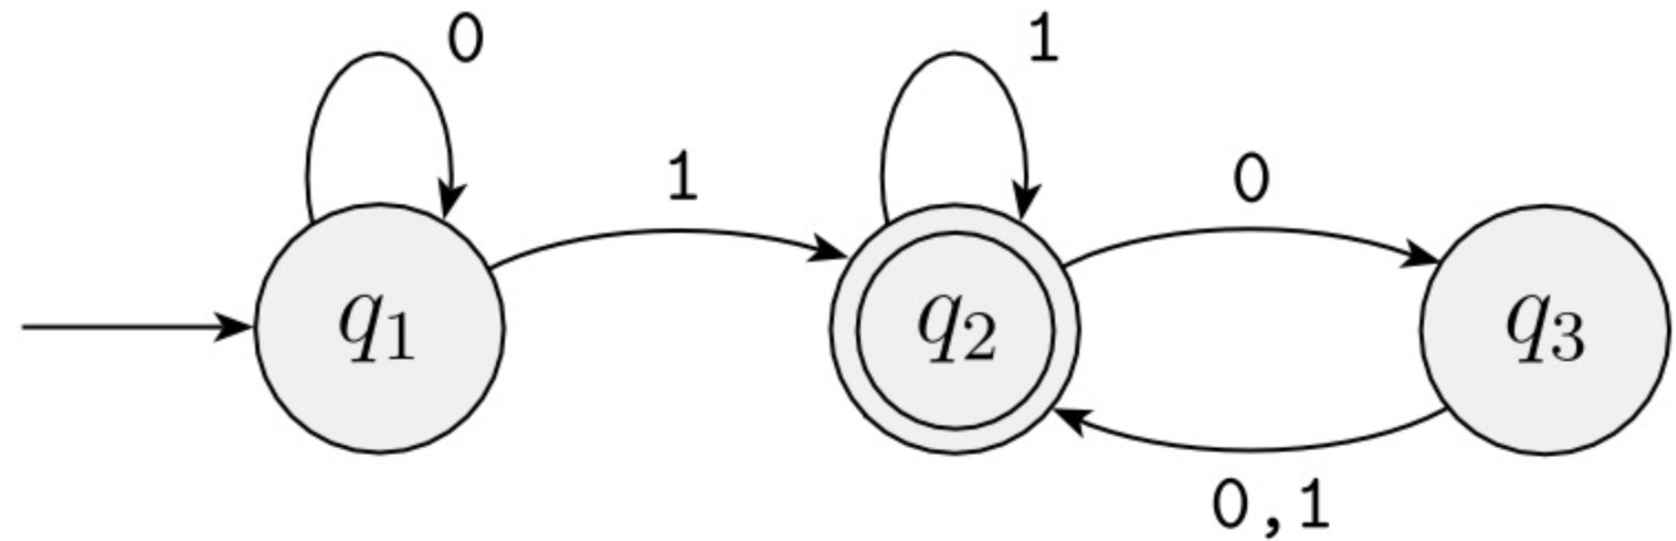
\includegraphics[scale = 0.25]{imgs/001.png}
    \end{center}
\end{example}

\noindent Automata change states depending on the string that they receive in input. So when a string $x$ is given to the automaton, it goes through the string symbol by symbol, and changes states depending on the input characters read and the result of the transition function. If, after reading the whole string, the automaton arrives at a final input, then we say that it \textbf{accepts} the string, otherwise it \textbf{rejects} it.

\begin{definition}{Language of an automaton and Regular Language}
    The \textbf{language of an automaton} $M$, denoted as $L(M)$, is the \textbf{set} of all those \textbf{input strings} which make the automaton \textbf{go} from the starting state \textbf{to} a \textbf{final state}.
    \\\\
    \noindent More specifically: given an automaton $M = (Q, \; \Sigma, \; \delta, \; q_{0}, \; F)$ and let $w$ be a string of $n$ symbols where $w_i$ denotes the $i^\text{th}$ symbol of the string; let also that
    \[ \forall \; w_{i} \in w, \text{ then } w_{i} \in \Sigma \]
    
    \noindent Then, we say that $M$ accepts $w$ if there exists a set of states $r = \{ r_{0}, \; r_{1}, \; \dots, \; r_{n} \} \in Q$ which respects all the following three conditions:
    \begin{itemize}
        \item $r_0 = q_0$: the first state of $r$ must coincide with the initial state;
        \item $\delta(r_{i}, \; w_{i + 1}) = r_{i + 1}, \; \forall  i \in [0, \; 1, \; \dots, \; n-1]$: each character must lead to a transition of state;
        \item $r_{n} \in F$: the final state in $r$ should be in $F$.
    \end{itemize}
    
    \noindent $M$ recognizes a language $A$ If
    \[ A = \{ w \; | \; M \text{ accepts } w \} \]

    \noindent A \textbf{language} $L$ is said to be \textbf{regular} if there exists a finite automaton $M$ which accepts $L$
\end{definition}

\noindent Note that it's possible for an automaton to have that $q_{0} \in F$.

\section{Non-Deterministic Finite Automata (NFA)}

With DFA, we always knew that, given a current state $q_i$ and a character $w_i \in \Sigma$, then we would \textbf{always know} what the \textbf{next state} would be. There is another type of automata which breaks this deterministic rule, and is called \textbf{non-deterministic finite automata}.

\begin{definition}{Non-Deterministic Finite Automaton (NFA)}
    A \textbf{non-deterministic finite automaton} (\textbf{NFA}) is an automaton denoted by a tuple of 5 elements $(Q, \; \Sigma, \; \delta, \; q_{0}, \; F)$ where:
    \begin{itemize}
        \item $Q$ is a finite set of \textbf{states} that the automaton can reach;
        \item $\Sigma$ denotes a finite \textbf{alphabet} recognized by the automaton;
        \item $\delta$ is the \textbf{transition function}, which given $Q$ and $\Sigma_\epsilon$ returns the \textbf{power set} of $Q$ (denoted by $\mathcal{P}(Q)$);
        \[ \delta \; : \; Q \times \Sigma_\epsilon \longmapsto \mathcal{P}(Q) \]

        \item $q_{0} \in Q$ is the \textbf{starting state} of the automaton;
        \item $F \subseteq Q$ is the set of \textbf{accepted states}.
    \end{itemize}

    \noindent The power set $\mathcal{P}(Q)$ of a set $Q$ is the set of all subsets of $Q$, for any $Q$; the alphabet denoted with $\Sigma_\epsilon$ is equal to $\Sigma \cup \{ \epsilon \}$.
\end{definition}

In practice, how do NFAs work? The idea of NFAs is that, at \textbf{any moment in time}, \textbf{several choices may exist} for deciding the next state, and also $\epsilon$ can be a choice. An NFA runs through an input in the following way:
\begin{itemize}
    \item [1)] Like for DFAs, we start from the initial state $q_0$;
    \item [2)] Let $q$ denote the current state and $a$ the next symbol that the NFA receives as input, then:
    \begin{itemize}
        \item [a)] For every $a$-transition, the machine \textbf{splits} into a \textbf{different copy} and follows the path given by $a$, in parallel with all the other possible copies that might have been created. For instance, if from a state we have three outgoing transitions $0 \rightarrow q_i$, $1 \rightarrow q_j$ and $1 \rightarrow q_k$, then the machine will split into three different copies and, in parallel, will proceed on the three states, and the procedure will go on for each state;
        \item [b)] For every $\epsilon$-transition, the machine will split itself into a new copy \textbf{without reading the input}, and then each copy will proceed from the destination state given by each $\epsilon$-transition;
        \item [c)] If a state $q$ has no outgoing transitions, and $q \notin F$, then that copy of the machine dies, alongside all its computations.
    \end{itemize}
    \item [3)] If \textbf{any of the copies} of the NFA arrives to a final state, then we say that the \textbf{NFA accepts} the input string.
\end{itemize}

We can think of an NFA as a machine that runs sort of "\textit{parallel}" computations on independent threads, concurrently. It's also possible to think of an NFA as a \textbf{tree}, where the root of the tree is the root of the computation, and where each branch represents a possible choice that the machine has. If at least one of the leafs of the tree is a final state, then the machine accepts the input. Let's better formalize the acceptance of an NFA:

\begin{definition}{Acceptance of an NFA}
    Let $N \eq (Q, \; \Sigma, \; \delta, \; q_0, \; F)$ be an NFA and $w$ a string over the alphabeth $\Sigma$. We say that $N$ \textbf{accepts} $w$ if $w$ can be rewritten as $w \eq y_1 y_2 ... y_m$ where $\forall i \in m, \; y_i \in \Sigma_{\epsilon}$ and there exists a sequence of states $r_0, \; r_1, \; ..., \; r_m$ in $Q$ such taht the following three conditions are respected:
    \begin{itemize}
        \item $r_0 \eq q_0$ the initial states must coincide;
        \item $r_{i + 1} \in \delta(r_i, \; y_{i + 1})$: the next state must be in the set of states returned by the transition function given a specific state $r_i$ and the next input character $y_{i + 1}$;
        \item $r_m \in F$: the final state must belong to $F$.
    \end{itemize}

    It is possible that $m \geq |w|$, because some $w_i \in w$ can be $\epsilon$.
\end{definition}

The possibility of using $\epsilon$ as a valid character is very helpful when it comes to recognizing one pattern of characters among a set of patterns. In the following example is better explained how to use this approach:

\begin{example}
    Suppose that we want to build an automaton (specifically, an NFA) which recognizes the words in the following language:
    \[ \left\{ \; 0^k \; : \; k \text{ is a multiple of 2 or 3 } \right\} \]

    How can we build such automaton? Let's break it down into two smaller parts:
    \begin{itemize}
        \item if $k$ must be a multiple of 2, then the automaton is as follows:
        \begin{center}
            \begin{tikzpicture}[shorten >= 1pt, node distance=3cm, on grid, auto, bend angle=30]
                \node[state, initial, accepting] (q_0) {$q_0$};
                \node[state] (q_1) [right of=q_0] {$q_1$};
                \path[->] 
                (q_0) edge [bend left] node {0} (q_1)
                (q_1) edge [bend left] node {0} (q_0);
            \end{tikzpicture}
        \end{center}

        \item if $k$ must be a multiple of 3, then the automaton is as follows:
        \begin{center}
            \begin{tikzpicture}[shorten >= 1pt, node distance=2cm, on grid, auto, bend angle=20]
                \node[state, initial, accepting] (q_0) {$q_0$};
                \node[state] (q_1) [above right of=q_0] {$q_1$};
                \node[state] (q_2) [below right of=q_0] {$q_2$};
                \path[->] 
                (q_0) edge [bend left] node {0} (q_1)
                (q_1) edge [bend left] node {0} (q_2)
                (q_2) edge [bend left] node {0} (q_0);
            \end{tikzpicture}
        \end{center}
    \end{itemize}

    We can merge these two automatons thanks to the $\epsilon$-transition. This way the automaton will create a copy of itself for both cases (so that $w$ has a number of zeroes which is either a multiple of 2 or 3, in the best case the number will be simultaneously a multiple of both 2 and 3), and if at least one of the two cases will end up in a final state, then the NFA will accept such string. Here is the final version:

    \begin{center}
        \begin{tikzpicture}[shorten >= 1pt, node distance=2cm, on grid, auto, bend angle=30]
            \node[state, initial] (s) {$s$};
            \node[state, accepting] (q_0) [above right of=s] {$q_0$};
            \node[state] (q_1) [right of=q_0] {$q_1$};
            \node[state, accepting] (q_2) [below right of=s] {$q_2$};
            \node[state] (q_3) [right of=q_2] {$q_3$};
            \node[state] (q_4) [right of=q_3] {$q_4$};
            \path[->] 
            (s) edge node {$\epsilon$} (q_0)
            (s) edge node {$\epsilon$} (q_2)
            (q_0) edge [bend left] node {0} (q_1)
            (q_1) edge [bend left] node {0} (q_0)
            (q_2) edge node {0} (q_3)
            (q_3) edge node {0} (q_4)
            (q_4) edge [bend left] node {0} (q_2);
        \end{tikzpicture}
    \end{center}
\end{example}

Intuitively, we may think that a DFA can be expressed with an NFA, since DFAs are a specific version of NFAs where there are no $\epsilon$-transitions and where, from each state, given a specific input character, there is only one possible action to perform. But can we say the same of the other way around? So, is there, for each NFA, the possibility to express is with a DFA? There is a theorem which states that it's possible, and we'll also see its proof:

\begin{theorem}{Equivalence of DFAs and NFAs}
    For every NFA $N$ there exists a DFA $M$ such that the language accepted by $N$ is also accepted by $M$ (so $L(N) \eq L(M)$)

    \begin{proof}
        Let $N$ be an NFA such that $N \eq \{Q, \; \Sigma, \; \delta, \; q_0, \; F \}$ and let $A \eq L(N)$ denote the language accepted by $N$. Our objective is to devise a DFA $M \eq \{Q', \; \Sigma, \; \delta', \; q_0', \; F' \}$ which accepts that same language $A$.
        \nl
        Let's first consider a case where the NFA has no $\epsilon$-transitions: 
    \end{proof}
\end{theorem}